\subsection{Подготовка данных}

Первый корпус был взят из работы \cite{aharoni2014benchmark}. Данный корпус состоит из размеченных тем и предпосылок. Всего в корпусе представлено 83 темы. В данном корпусе пары размечены бинарным отношением  наличия релевантности, при этом под релевантностью подразумевается исключительно поддержка, т.е. в рамках данной постановки задачи предпосылки, противоречащие утверждению, имеют тот же класс, что и предпосылки, не имеющие никакого отношения к утверждению. Пример утверждения, относящегося к теме:
\begin{verbatim}
Утверждение: We should increase gun control
Обоснование: Gun control laws are depicted as benign and 
historically progressive.
\end{verbatim}

Для исследования возможности переноса знаний между языками данный корпус был переведен на русский язык.

Так как идейно в этой задаче моделируется связь между двумя высказываниями было решено адаптировать корпуса из задачи Textual Entailment (Natural Language Inference). Был адаптирован русскоязычный корпус TERRa, состоящий из гипотез и предпосылок, которые очень близки к предыдущему корпусу. Пример связанной гипотези и предпосылки:
\begin{verbatim}
Предпосылка: Автор поста написал в комментарии, 
что прорвалась канализация.
Гипотеза: Автор поста написал про канализацию.
\end{verbatim}

У данной постановки задачи существуствует один важный недостаток - она не позволяет различить нейтральную связь от атакующей. Для этого был адаптирован корпус \cite{bar2017stance}, позволяющий определить полемическую позицию аргументации. В данном  корпусе размечены аналогичные пары утверждений и предпосылок в отношения атаки и поддержки. В данном корпусе отсутствуют нейтральные отношения. Для этого были дополнительно обработаны размеченные тексты, и все тексты, не размеченные в поддержку или атаку считались нейтральными. Пример:
\begin{verbatim}
Утверждение: Реклама вредна
Предпосылка: Реклама распространяет консьюмеризм и культуру потребительства
Вид связи: Поддержка

Утверждение: Бокс полезен
Предпосылка: Бокс остается 8м самым летальным видом спорта
Вид связи: Атака
\end{verbatim}

\subsection{Обучение моделей}
\subsubsection{Поиск предпосылки по утверждениям}

Было проведено несколько различных экспериментов. Исследовалась переносимость знаний на русский язык и влияние стороннего корпуса на эффективность переноса знаний. Обучение и валидация происходили на англоязычной версии корпуса. Были обучены следующие вариации моделей:
\begin{itemize}
    \item combined\_mbert\_frozen - мультиязычная модель, обученная на корпусе TERRa и корпусе IBM Evidence Search.
    \item ibm\_mbert\_frozen - мультиязычная модель, обученная на корпусе IBM Evidence Search.
    \item terra\_mbert\_frozen - мультиязычная модель, обученная на корпусе TERRa.
\end{itemize}

Как видно из графиков обучения, лучше всего работает модель ibm\_mbert\_frozen. Как и все названные модели она базируется на модели multilingual BERT. При обучении для применения техники crosslingual transfer у модели замораживается матрица эмбеддингов.

На англоязычной тестовой выборке модели показывают F1-меру около 0.75. При переходе на переведенную русскоязычную версию корпуса качество падает до 0.72-0.75, что говорит об успешном переносе знаний.

Стоит отметить, что на этом корпусе нет установленной таблицы лидеров, поэтому заявленные числа тяжело оценить из-за отсутствия каких-либо конкурентов. Однако ранее упомянутая система MARGOT заявляет об F1-мере в 0.3. Подробные примеры работы можно увидеть в приложении.

\begin{figure}[h!]
  \centering
  \begin{minipage}[b]{0.45\textwidth}
    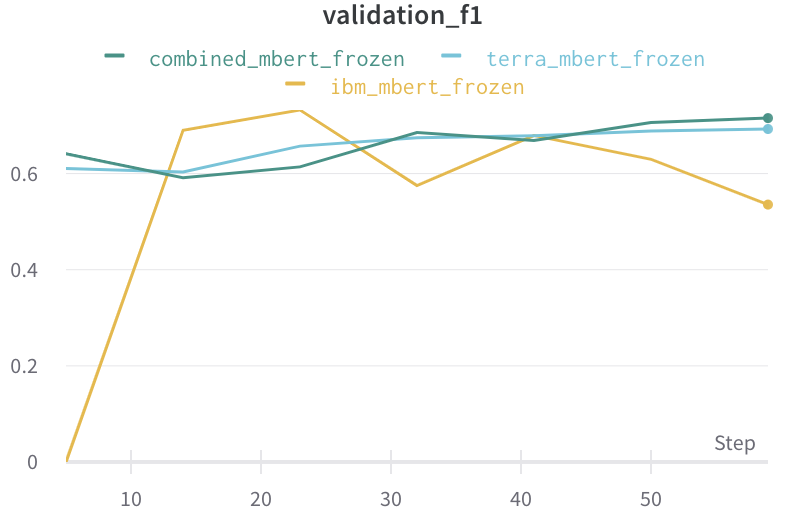
\includegraphics[width=\textwidth]{f1.png}
    \caption{F1-мера}
  \end{minipage}
  \hfill
  \begin{minipage}[b]{0.45\textwidth}
    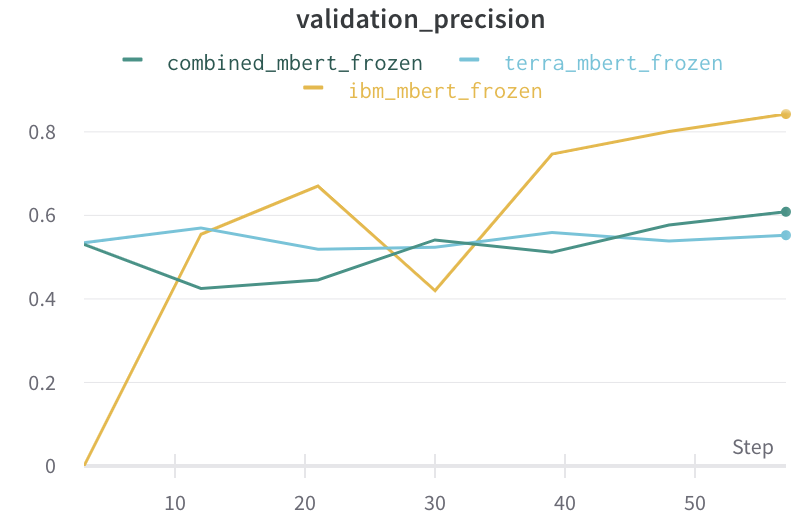
\includegraphics[width=\textwidth]{precision.png}
    \caption{Точность}
  \end{minipage}
  \begin{minipage}[b]{0.45\textwidth}
    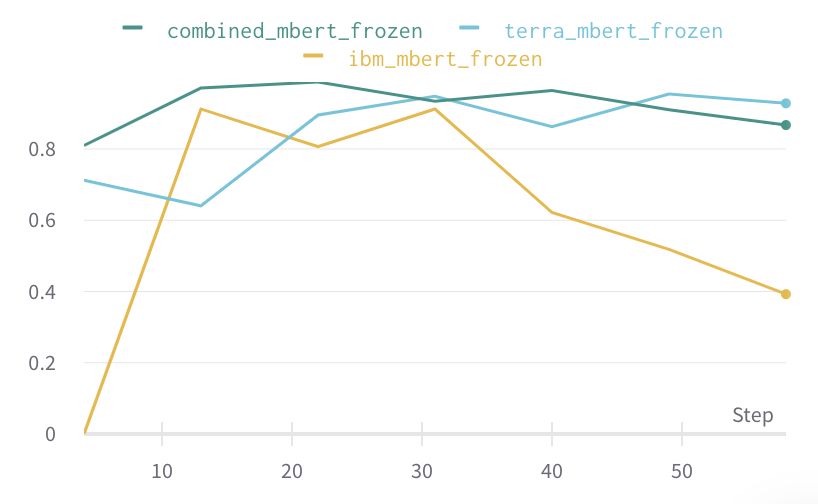
\includegraphics[width=\textwidth]{recall.png}
    \caption{Полнота}
    \label{pd_3}
  \end{minipage}
\end{figure}

\subsubsection{Классификация предпосылок}
Задача классификации предпосылок также была расширена так, как это описано в обработке данных. Вместо задачи бинарной классификации в отношения атаки и поддержки рассматривается задача регрессии в отрезок $[-1; 1]$, где -1 - атака, 1 - поддержка, 0 - нейтральное отношение. Для получения классов данный отрезок был поделен на 3 равные части. По этим частям считалась точность, предоставленная на соответствующем графике.

\begin{figure}[H]
 \captionsetup{justification=raggedright,singlelinecheck=false,labelfont=bf,labelsep=period,name={Рисунок}}
 \centering{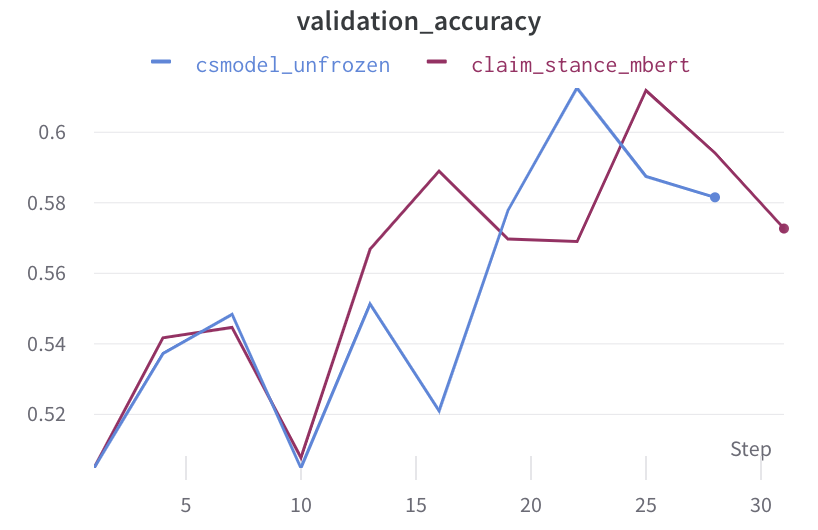
\includegraphics[scale=0.55]{accuracy.png}}
 \caption{Точность системы классификации полемической позиции предпосылок по отношению к утверждениям.}
\end{figure}

Стоит отметить, что в задачах очень сильные сдвиги в распределениях - нейтральных примеров много больше, чем положительных или отрицтательных.

\subsection{Обнаружение пропаганды}

Как отмечалось ранее, пропаганда является политической аргументацией. Было принято участие в соревновании  SemEval 2020 Task 11 Propaganda Detection In News Articles\cite{da2020semeval}. Было представлена два трека - детекция пропаганды и классификация пропаганды. По результатам\cite{dimov-etal-2020-nopropaganda} участия было занято 7 место из 36 в первом треке и 6 из 31 во втором треке.

Корпус состоял из ручной разметки новостных статей за 2019 год. Всего было обработано 438 статей, содержащих 21230 предложений, из которых 7485 содержали пропаганду.

\subsubsection{Определение участков текста с пропагандой}
В первом треке требовалось определить участки текста, являющиеся пропагандой, т.е. постановка задачи заключается в бинарной разметке текста на предмет наличия приемов убеждения. 

\begin{figure}[H]
 \captionsetup{justification=raggedright,singlelinecheck=false,labelfont=bf,labelsep=period,name={Рисунок}}
 \centering{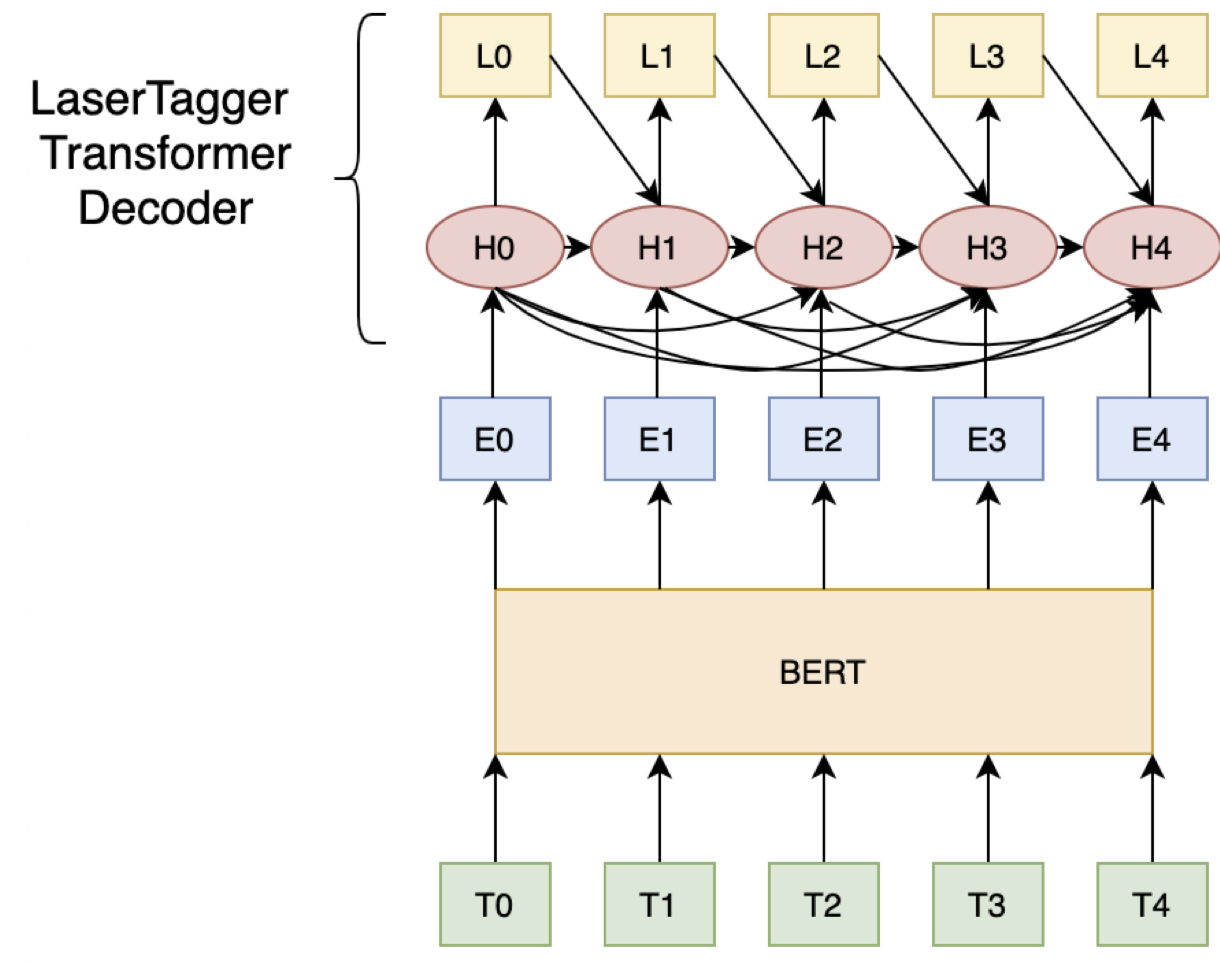
\includegraphics[scale=0.5]{lasertagger.png}}
 \caption{Архитектура LaserTagger из первого трека. $T_i$ - входная последовательность токенов, $L_i$ - бинарные метки для токенов.}
\end{figure}

Т.к. задача тэгирования последовательности, частным видом которой является распознавание именованных суностей, имеет ряд стандартных архитектур, было решено применить несколько стандартных подходов для получения хорошего базового решения.

\begin{figure}[H]
\setcounter{figure}{0}
 \captionsetup{justification=raggedright,singlelinecheck=false,labelfont=bf,labelsep=period,name={Таблица}}
 \centering{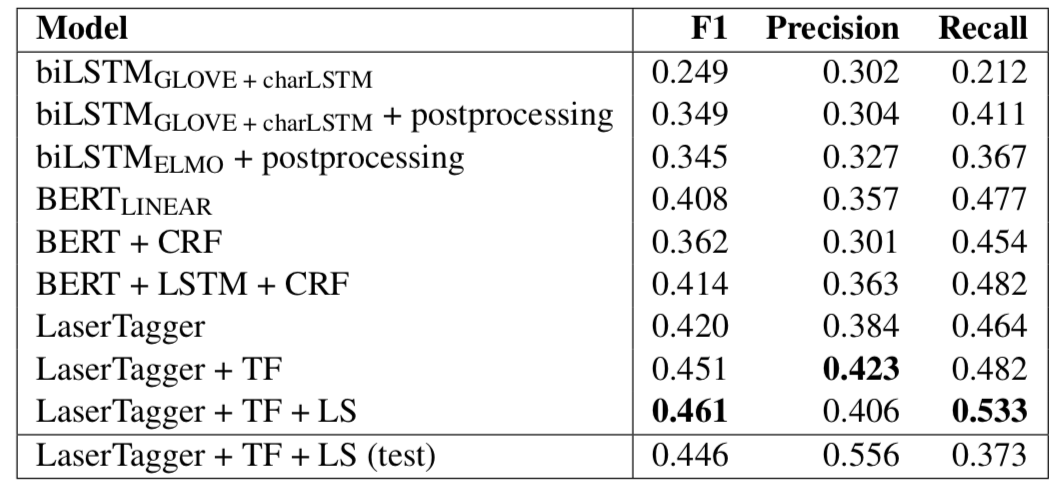
\includegraphics[scale=0.7]{laser_table.png}}
 \caption{Архитектура LaserTagger из первого трека. $T_i$ - входная последовательность токенов, $L_i$ - бинарные метки для токенов.}
\end{figure}

В результате была принята авторегрессионная модель LaserTagger \cite{malmi2019encode}. По сравнению с обычными моделями тэгирования у нее есть одно важное преимущество: она учитывает свои предыдущие предсказания, поэтому она имеет возможность предсказывать длинные непрервыные участки текста без разрывов.

Как видно из таблицы стандартные пододы получают низкие метрики в районе 24-35\% F1-меры. Использование CRF для связного предсказания меток не приносит пользы. Базовая модель, основанная на BERT сразу получает метрику в 40\%.

Для обучения финальной версии архитектуры lasertagger использовалась методика labelsmoothing для смягчения ошибок по краям пропаганды, а также teacher forcing. Teacher forcing заключается в смешивании результатов авторегресионной модели с ее предсказаниями во время обучения. Таким образом получается, что модель ошибается во время обучения и ислледуюет больше пространства и становится более устойчивой к ошибкам.

Анализ ошибок показал, что данная модель имеет и некоторые недостатки: модель часто выделяет различные обособленные обороты и цитаты полностью, вместо их частей. Также модель иногда наоборот закрывает участок с пропагандой при переходе через запятую и не открывает участок заново.

Часть проблем возникает и из-за особенностей корпуса. В корпусе прослеживается сильное смещение тем между тестовой выборкой и тренировочной, валидационной. Из-за этого метрики всех участников на валидационной выборке на 10-15\% выше, чем итоговые результаты на тесте.
